\documentclass[10pt]{article}
\usepackage[utf8]{inputenc}
\usepackage[T1]{fontenc}
\usepackage{graphicx}
\usepackage[export]{adjustbox}
\graphicspath{ {./images/} }
\usepackage{amsmath}
\usepackage{amsfonts}
\usepackage{amssymb}
\usepackage[version=4]{mhchem}
\usepackage{stmaryrd}

\title{Intermediate Assignment 
 Level Control for Three-Tank System }

\author{}
\date{}


\begin{document}
\maketitle
\section*{1 System Description}
Fluid flow systems, hence liquid level control, are very common in process control. Typical industrial applications are wastewater treatment, petro/chemical plants, and oil/gas facilities. The three-tank system in Figure 1 can be viewed as a case study representing such a fluid flow system.

\begin{center}
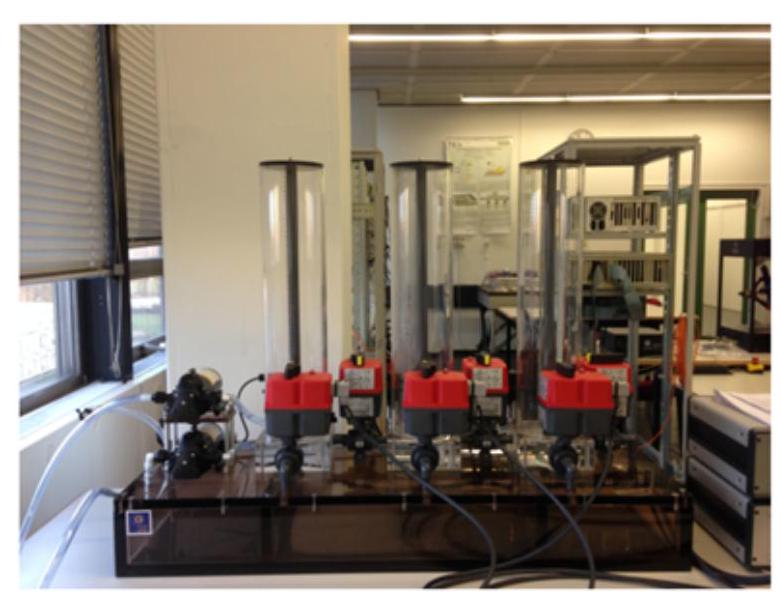
\includegraphics[max width=\textwidth]{2023_11_30_1daa78c814c553452d7bg-1(1)}
\end{center}

Figure 1: Three tank system

\begin{center}
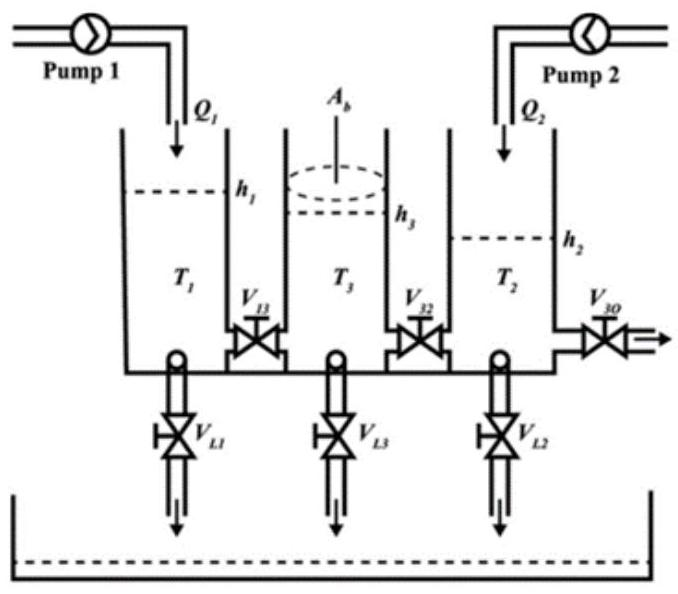
\includegraphics[max width=\textwidth]{2023_11_30_1daa78c814c553452d7bg-1}
\end{center}

Figure 2: Schematic representation of the system

In Figure 2 depicting the schematic representation of the real system, the plant mainly consists of the following components:

\begin{itemize}
  \item Three plexiglass cylinders labeled by $T_{1}, T_{2}$, and $T_{3}$ (left, right and middle tank) with the same cross-sectional area $A_{b}$;
  \item Pump 1 and 2 that pumps water from the reservoir to $T_{1}$ and $T_{2}$ respectively;
  \item Six adjustable valves including $V_{13}$ and $V_{32}$ that control the interconnected flows between corresponding tanks, $V_{L 1}, V_{L 2}$, and $V_{L 3}$ simulating tank leaks, and $V_{30}$ that controls the output flow;
  \item A reservoir on the bottom.
\end{itemize}

Furthermore, the following notations are used to represent the system:

\begin{itemize}
  \item $h_{1}, h_{2}$, and $h_{3}$ respectively denote the liquid heights of the three tanks $T_{1}, T_{2}$, and $T_{3}$;
  \item $Q_{1}$ and $Q_{2}$ are the flow rates $(L / s)$ of the pumps 1 and 2 .
  \item The pipe flow controlled by valves $V_{13}$ and $V_{32}$ are respectively denoted by $q_{13}$ and $q_{32}$, and The leakage flows are denoted by $q_{1}, q_{2}$, and $q_{3}$, respectively. In addition, $z_{i} \in[0,1]$ represents the opening rate of corresponding valves with $i$ index.
\end{itemize}

More detailed parameters and descriptions can be found in the manual [1].

\section*{2 System Model}
A normal task for the three-tank system is to control the liquid levels of tanks to desired heights. In this assignment, the valve of output flow $V_{30}$ is completely closed. In fact, the system $\dot{x}=f(x, u)$ is a nonlinear system. The state of the system is denoted by $x=\left[h_{1}, h_{2}, h_{3}\right]$, which can be measured via sensors in real time (unit: $\mathrm{mm}$ ). From the Bernoulli's principle, the dynamic system of the liquid level can be expressed with the following equations,

$$
\begin{gathered}
\frac{d h_{1}}{d t}=\frac{1}{A_{b}}\left(Q_{1}-q_{13}-q_{1}\right)=\alpha p_{1}-k_{13} \sqrt{\left|h_{1}-h_{3}\right|} \operatorname{sign}\left(h_{1}-h_{3}\right)-k_{1} \sqrt{h_{1}} \\
\frac{d h_{2}}{d t}=\frac{1}{A_{b}}\left(Q_{2}-q_{23}-q_{2}\right)=\alpha p_{2}-k_{23} \sqrt{\left|h_{2}-h_{3}\right|} \operatorname{sign}\left(h_{2}-h_{3}\right)-k_{2} \sqrt{h_{2}} \\
\frac{d h_{3}}{d t}=\frac{1}{A_{b}}\left(q_{13}+q_{23}-q_{3}\right)=k_{13} \sqrt{\left|h_{1}-h_{3}\right|} \operatorname{sign}\left(h_{1}-h_{3}\right)+k_{23} \sqrt{\left|h_{2}-h_{3}\right|} \operatorname{sign}\left(h_{2}-h_{3}\right)-k_{3} \sqrt{h_{3}}
\end{gathered}
$$

where $p_{1}$ and $p_{2}$ denote the input voltages of the corresponding pumps, which are propositional to flow rate $Q_{1}$ and $Q_{2}$ with the constant $\alpha$, respectively. $k_{i}$ is a variable characterizing the flow rate of the $i$-th valve with respect to its opening rate $z_{i}$. In the real system, there is a nonlinear relationship between $k_{i}$ and $z_{i}$, such as an identified model based on sigmoid function [2]. For the sake of simplicity, $k_{i}$ are directly used as the control inputs rather than corresponding $z_{i}$ in this assignment. Therefore, the control inputs of the system includes $p_{1}, p_{2}, k_{1}, k_{2}, k_{3}, k_{13}, k_{23}$.

\section*{3 Questions}
Given the above brief introduction to the three-tank systems, you are expected to solve the following problems step by step.

(1) Linearization for the single-tank system Consider a single tank system $T_{1}$ with initial state $h_{1}(0)=0$ where the interconnected valve $V_{13}$ is closed and the opening rate of $V_{L 1}$ is set as $z_{1}=0.3$. The dynamic equation of the single tank systems is as follows,

$$
\frac{d h_{1}}{d t}=\frac{1}{A_{b}}\left(Q_{1}-q_{1}\right)=6.5 p_{1}-0.07 \sqrt{h_{1}}
$$

As for the system with $x=h_{1}$ and $u=p_{1}$, linearize the single tank system around the steady state $h_{1}=300 \mathrm{~mm}$. Note that the detailed derivation procedure should be attached.

(2) Controller design for the three-tank system: In the task, consider the complete three-tank system with the initial state $h_{1}(0)=h_{2}(0)=h_{3}(0)=0$. The opening rates of leakage valves including $V_{L 1}, V_{L 2}$, and $V_{L 3}$ are set as $z_{1}=z_{2}=z_{3}=0.5$. Therefore, the control input is $u=$ $\left[p_{1}, p_{2}, k_{13}, k_{32}\right]$. The discrete-time linearized system around the steady state $x^{*}=[450,400,350]$ and steady-state input values $u^{*}=[0.9627,0.7556,0.2166,0.2074]$ is provided as follows,

$$
\begin{gathered}
\xi(k+1)=A \xi(k)+B \mu(k) \\
A=\left[\begin{array}{cccc}
0.9987 & 0 & 0.0009 \\
0 & 0.9988 & 0.0011 \\
0.0009 & 0.0011 & 0.9975
\end{array}\right] \\
B=\left[\begin{array}{cccc}
0.6524 & 0 & -0.9989 & 0.0003 \\
0 & 0.7076 & 0.0006 & -0.7063 \\
0.0003 & 0.0004 & 0.9983 & 0.7055
\end{array}\right]
\end{gathered}
$$

where $x(k)=x^{*}+\xi(k), u(k)=u^{*}+\mu(k)$, and the time step $\Delta t=0.1 \mathrm{~s}$. In the linearized system, sign() operators in Equation (1) are eliminated due to the assumption that the heights of $T_{1}$ (left tank) and $T_{2}$ (right tank) are higher than $T_{3}$ (middle tank) in the process.

\begin{itemize}
  \item Given the desired pole $[-2,-2,-2]$, design a controller to stabilize the linearized system with the pole placement method.
  \item Given the diagonal matrix $Q=\operatorname{diag}(2,2,2)$ and $R=\operatorname{diag}(0.1,0.1,1,1)$, design a LQR controller for the system.
\end{itemize}

Please verify the designed controller first on the simulation based on the provided linearized system, and plot the related state profiles over time. And then, deploy the controller on the RemoteLab platform [3], where the real-time response of the three-tank system can be observed via the camera and sensors. You are encouraged to try different desired poles and weight matrix, and briefly analyze the performance difference. Please attach the necessary derivation procedure and the analysis for the obtained experimental data in your report.

Tips: 1) Leverage Matlab functions place() and $\operatorname{lpr}($ ) to design controller; 2) You just need to fill in the Controller block of the Simulink file, and then upload zip file to the RemoteLab. Note that the Simulink file should be saved as an old version, like 2019b.

\section*{References}
[1] Control System Group, "Three-Tank-System operator manual," 2016.

[2] P. Chalupa, J. Novák, and V. Bobál, "Mathematical model of control valves of three-tank system," International Journal of Mechanics, 2011.

[3] Control System Group, "RemoteLabs User Manual," 2021.


\end{document}